\documentclass[12pt,a4paper]{article}
\usepackage[utf8]{inputenc}
\usepackage[T1]{fontenc}
\usepackage{amsmath, amssymb, amsthm}
\usepackage{geometry}
\usepackage{fancyhdr}
\usepackage{enumitem}
\usepackage{tikz}
\usepackage{animate}

\usepackage{blindtext}
\usepackage[hidelinks]{hyperref}
\usepackage{setspace}
\usepackage{float}
\usepackage{pdfpages}
\usepackage[hypcap=true]{caption}
\hypersetup{hypertexnames=false} % Fixes duplicate identifier warnings
\usepackage{minted}
\usepackage[export]{adjustbox}

\definecolor{pastelred}{HTML}{FF7F7F}
\definecolor{pastelblue}{HTML}{9999FF}
\definecolor{pastelgreen}{HTML}{A8FFA8}

\setminted{
    breaklines=true,
    fontsize=\small,
    xleftmargin=0pt
}

\usepackage{comment}
\usetikzlibrary{calc,shapes.multipart,positioning,decorations.pathreplacing,arrows.meta}
\hypersetup{
    colorlinks=true,
    linkcolor=blue,
    filecolor=magenta,      
    urlcolor=cyan,
    pdfpagemode=FullScreen,
    }

\urlstyle{same}

\usepackage[most]{tcolorbox} % For the pretty terminal box
\newtcolorbox{terminalbox}{
    colback=gray!5!white,
    colframe=gray!40!white,
    fontupper=\small\ttfamily,
    sharp corners,
    boxrule=0.5pt,
    width=\linewidth,
    halign=left
}

\singlespacing{}

\setlength{\parindent}{0pt}
\setlength{\parskip}{0.5\baselineskip}

% Page Layout
\geometry{margin=1in}
\pagestyle{fancy}
\fancyhf{}
\lhead{CSE306 project 2 report}
\rhead{CSE306 EP}
\cfoot{\thepage}

\begin{document}

\title{\textbf{CSE306 project 2 report}}
\author{Cristian Verde}
\date{}
\maketitle

\section{Overview}

The objective of this project was to write a 2D fluid simulator using Voronoï cells and the Euler equations for incompressible liquids.

Originally, for $N$ particles, we computed their Voronoï cells (regions in which they are the closest point by Euclidean distance). Afterwards, we had to balance the cells (have them have equal surface area) using a Power (Laguerre) diagram --- each particle gets assigned a weight which basically transforms it into a circle, and the regions are made of points closest to a particle's circle. Since the weights can be arbitrary, a particle's region can be far from the particle itself based on the Euclidean distance. We had a functional to minimize, for which we used the LBFGS algorithm. For the $3^{\text{rd}}$ part, we adapted the formula to include air, clipped every ``water'' cell with an ``air'' disk, and ran a particle simulation based on the rules of Physics: apart from gravity, we add a spring force which pulls particles towards the center of their Voronoï cell (which, again, can be far away Euclideanly).

The only optional work I did was the addition of the kNN-search for closest neighbours using KD trees through the nanoFlann library. Using this, instead of comparing against all the other particles, we can compare only to some ``closest'' neighbours (defined based on a distance not necessarily Euclidean). It was done outside of the lab.

\section{Results}

The following images (and mp4) were generated on my local machine running an Intel i7-13700H with 14 cores (6 fast with 2 threads each and 8 with only 1 thread, totalling 20 threads). The compilation flags relevant for performance were \texttt{-O3 -fopenmp -ffast-math}.

\subsection{Lab 6}

\begin{figure}[H]
	\centering
	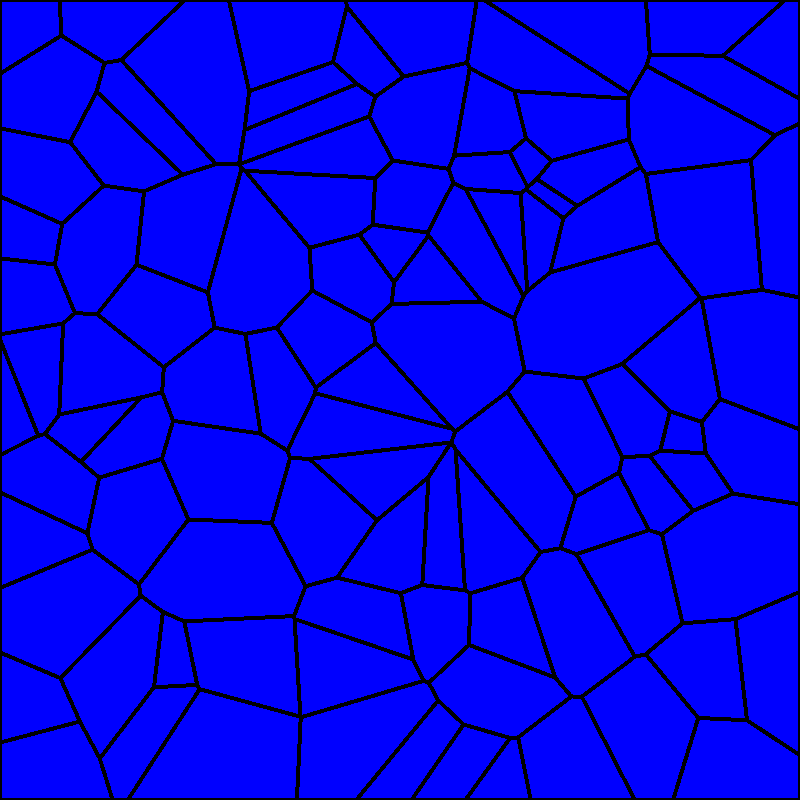
\includegraphics[width=0.5\textwidth]{../voronoi_pre_optim0.png}
	\caption{Result at the end of lab 1.}
\end{figure}

There is not much to say about this one. We select $100$ points uniformly in the $[0, 1]^2$ square, and then for each, we clip a square (which is initially $[0, 1]^2$) by the bisector of the segment between that point and its closest $30$ neighbours (less than this is needed for normal Euclidean distance, but once the weights are added it increases).

\subsection{Lab 7}

\begin{figure}[H]
	\centering
	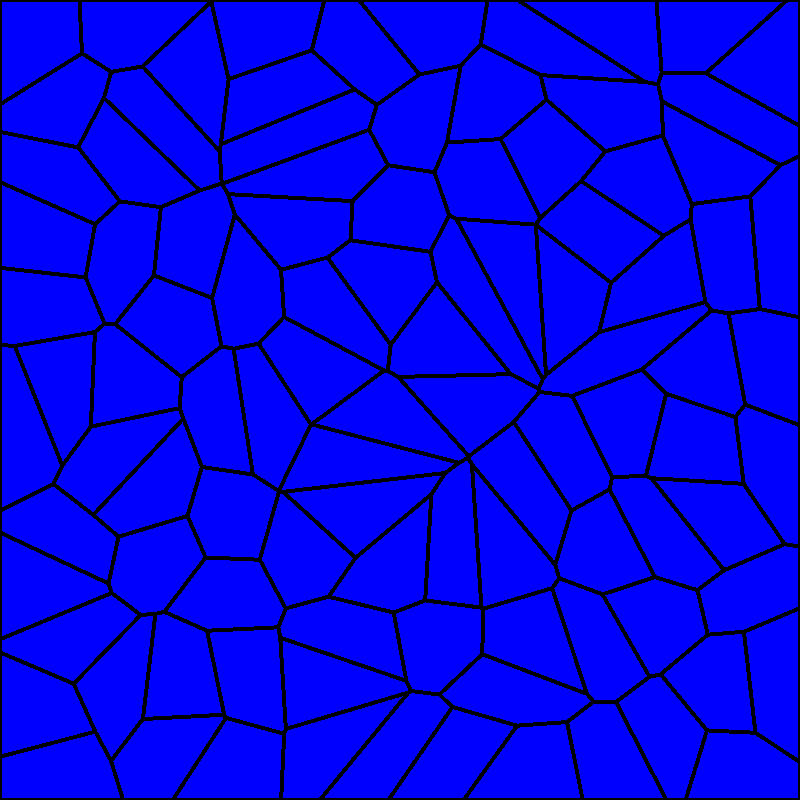
\includegraphics[width=0.5\textwidth]{../voronoi_optim0.png}
	\caption{Result at the end of lab 2.}
\end{figure}

As we can see, the cells now have roughly the same surface. The only change was that the squared distance from a random point $X$ to one of our points $P_i$ is $\|X - P_i\|^2 - w_i$. We can ``artificially'' add this weight in the $z$ coordinate of our points so that the kNN-search uses it. We then have to minimize the functional:
\[
	f(W) = -\left(\sum_{i} \int_{Pow_{W}(y_{i})} (\|x - y_{i}\|^2 - w_{i}) \mathrm{d}x + \sum_{i} \lambda_{i} w_{i}\right)
\]
where $\lambda_{i} = \frac{1}{N_{particles}}$ is the desired ``weight'' (area in our case, since the whole image has area $1$) of the cell. LBFGS just needs the current value of the function and its gradient, which are easily computable. At the end, using the obtained weights and our new distance logic, we generate the figure with almost equally large cells.

\subsection{Lab 8}

\begin{figure}[H]
	\centering
	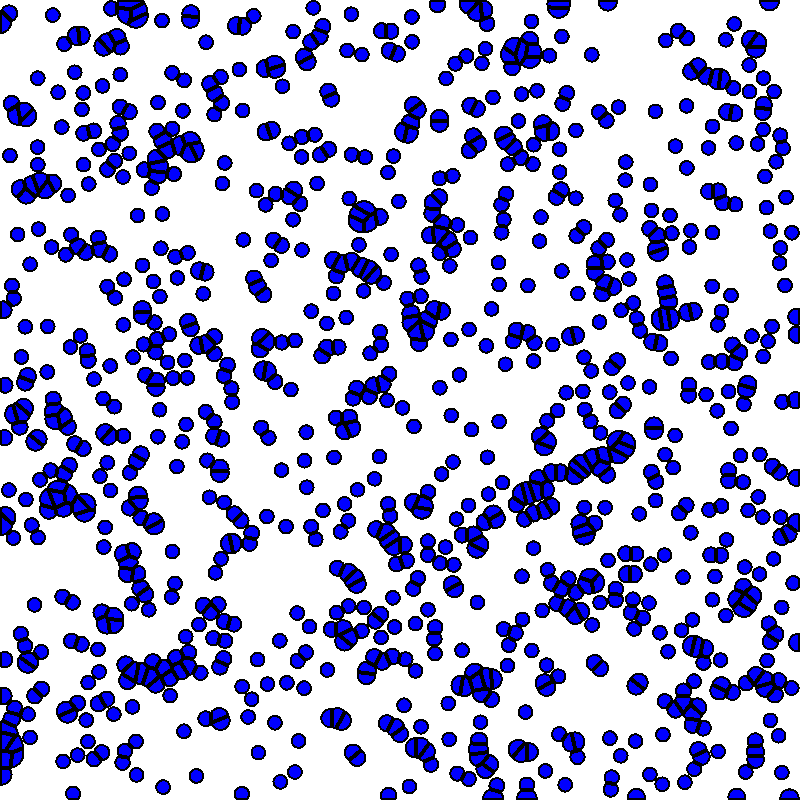
\includegraphics[width=0.7\textwidth, frame]{../fluid_video/frame_0.png}
	\caption{Starting configuration of liquid.}
\end{figure}

For this, we add a fictitious $w_{air}$ at the end of the weights vector and adapt the formulas to consider the effect of air: first, the cells are clipped by a disk of size $\sqrt{w_i - w_{air}}$ if $w_i > w_{air}$, which effectively sets a lower bound on the cell size and stops it from growing until the edges of the image. We can imagine it as the implementation of air pressure. We then just simulate the particles moving for a small amount of time according to gravity and a force pulling them towards the center of their Power cell, then recompute the Voronoï cells warmly (using the already-computed weights, since they are very good approximations for the weights at the next step so LBFGS will converge faster).

For some measurements, using $700$ particles occupying a disk of radius $0.3$ leading to $\pi 0.3^2 \approx 30\%$ water volume, $1000$ frames and comparing with $200$ neighbours, and clipping by a regular polygon with $50$ vertices, the running time is:

\begin{terminalbox}
	real    12m22.022s\\
	user    189m43.430s\\
	sys     1m12.968s
\end{terminalbox}

This is $\approx 0.72$s per frame, which is under the desired outcome of $1$s.

The video is available in the repository. It was generated with $1000$ particles, $300$ neighbours checked in the kNN-search, same radius $0.3$, $60$fps and $dt = 0.01$ so it moves pretty fast.

\subsection{Potential improvements}

As was suggested, this project could have been done in 3D or with a Newtonian solver (instead of a quasi-Newtonian one). As for performance, it runs pretty smoothly, the only parameter that can reduce computation is the number of neighbours which could be fine-tuned. Additionally, we could compute a dynamic number of neighbours instead of hard-coding a value (having $30$ instead of $200$ neighbours for $700$ particles was a bug I had, which made me lose my mind as I had no idea why my animation was weird).

\end{document}
